This section discusses the handling, parsing and validation of imported and exported .csv files.\par
\subsubsection{Use-cases}
The file handling module provides services to import, export and validate subject set files in .CSV format.\par
\begin{figure}[H]
    \centering
    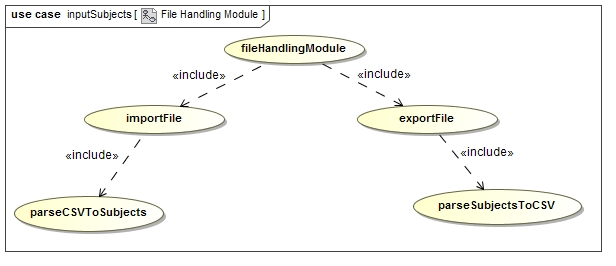
\includegraphics[width=15cm]{./graphics/fileUseCase.jpg}
    \caption{File Handling Module Use Case}
\end{figure}
\begin{enumerate}
\item parseCSVToSubjects\par
Priority: Critical\par
Pre-condition: The input file must pass the validation tests.\par
Post-condition: Subject set is modified locally.\par
\item saveSubjectsToDatabase\par
Priority: Critical.\par
Pre-condition: The user must click on the save button.\par
Pre-condition: The subject set needs to be locally modified.\par
Post-condition: The subject set is saved to the database.\par
\item parseSubjectsToCSV\par
Priority: Critical.\par
Pre-condition: The subject set must exist in the database.\par
Pre-condition: The correct format should be generated.\par
Pre-condition: The user must have enough hard disk space to save the .CSV file.\par
Post-condition: A CSV file with all the subjects existing in the project is downloaded to the user's hard drive .\par

\end{enumerate}